\section{Durchführung}
\label{sec:Durchführung}
Die Messungen wurden mit dem in \autoref{fig:aufbau} dargestellten Versuchsaufbau durchgeführt. 
\begin{figure}[H]
	\centering
	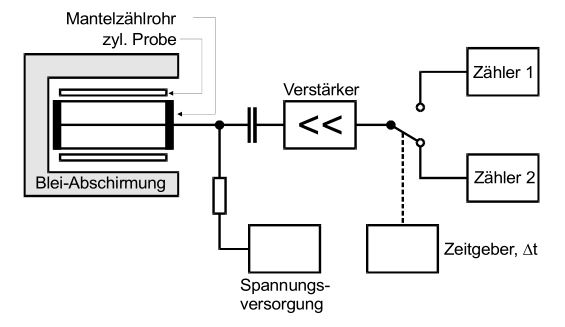
\includegraphics[width=0.8\textwidth]{content/aufbau.JPG}
	\caption{Versuchsaufbau \cite{sample}}
	\label{fig:aufbau}
\end{figure} 
Das Geiger-Müller-Zählrohr wird hier mit einem Abschirmblock aus Blei umgeben, um den Einfluss der Umgebungsradioaktivität zu minimieren. Der Zeitgeber dient dazu die Messzeit $\Delta t$ einzustellen. Dabei wird immer am Ende des Intervalls $\Delta t$ von einem Zähler auf den anderen umgeschaltet.
Vor der Zerfallsmessung muss außerdem der Nulleffekt $N_u$ gemessen werden, der durch Höhenstrahlung und natürliche Radioaktivität entsteht.